\flowchapter{Proposisjonar}{proposisjonar}

\begin{widebody}
\begin{center}\footnotesize
\begin{tabular}{@{}lllll@{}}
\textbf{\textit{d}} definisjon & \textbf{\textit{a}} postulat & \textbf{\textit{t}} teorem & \textbf{\textit{o}} observasjon & \textbf{\textit{i}} illustrasjon \\
\end{tabular}
\end{center}
\end{widebody}
\vspace{-4pt}

\mainprop{1}{}{Formverda er alt som er tilfelle.}

\prop{1.1}{o}{Formverda er totaliteten av realiserte konfigurasjonar, ikkje ting. Alt som har form, har eksakt denne forma. At noko tek éi form framfor ei anna, krev ei forklaring.}

\prop{1.2}{d}{Eit \textbf{objekt} er den enklaste bestanddelen i ei form. Objektet er udeleleg innanfor det valde analysenivået; det utgjer substansen i formverda. Alle moglege former er gjevne med objekta.}

\prop{1.21}{d}{Ein \textbf{konfigurasjon} er ei samansetjing av objekt. Forma er strukturen til konfigurasjonen.}

\prop{1.3}{d}{\textbf{Formrommet} (\textit{morphospace}) til ein klasse er mengda av alle hennar moglege konfigurasjonar.\textsuperscript{2,\,10,\,20} Kvart realisert objekt okkuperer eitt punkt i dette rommet. Det empiriske formrommet er alltid ein projeksjon; forma eksisterer uavhengig av målinga.}

\prop{1.31}{d}{Klassen avgrensar formrommet gjennom delt \textit{affordansestruktur}.\textsuperscript{12} Objekta i klassen tilbyr same konstellasjon av operasjonar til same konstellasjon av agentar. Klassen set grensene; seleksjonstrykket fordelar innhaldet.}

\prop{1.32}{d}{Formrommet er ein algebra lukka under union, differanse og transformasjon.\textsuperscript{11,\,13,\,18} Algebraen definerer kva operasjonar som er moglege.}

\propcont{Lat S vere ei mengd av former i eit euklidsk rom E\textsuperscript{n}, utstyrt med den euklidske transformasjonsgruppa Trans(E\textsuperscript{n}):}

\begin{center}\small
\begin{tabular}{@{}p{20mm}@{\hspace{3mm}}l@{\hspace{5mm}}p{30mm}@{}}
\textbf{Addisjon} & s\textsubscript{1} + s\textsubscript{2} & Legg til ein ny del; behald den opphavlege \\[5pt]
\textbf{Subtraksjon} & s\textsubscript{1} \msym{−} s\textsubscript{2} & Fjern ein del \\[5pt]
\textbf{Snitt} & s\textsubscript{1} \msym{·} s\textsubscript{2} & Del forma; behald omrisset \\[5pt]
\textbf{Innleiring} & \msym{τ}(a) \msym{≤} s & Finn ei delform i forma; endre proporsjon, orientering, retning \\
\end{tabular}
\end{center}

\propcont{Ei \textit{innleiring} av a i s er ein transformasjon som plasserer a i s, eventuelt rotert, flytta eller skalert. Innleiringa er ein eigenskap ved den noverande forma, uavhengig av korleis ho vart konstruert.}

\prop{1.4}{d}{Formrommet deler seg i tre regionar; \textit{busette}, \textit{opne} og \textit{forbodne}.}

\prop{1.41}{o}{Dei busette regionane er det historiske arkivet. Dei fungerer som ankerpunkt; tyngda veks med okkupasjonstid. Uavhengig konvergens stadfestar at attraktoren er reell.}

\prop{1.42}{o}{Dei opne regionane er det \textit{nærliggande moglege}. Tilgjengelege, men uaktualiserte. Dei er endelige; spente ut mellom det busette og det forbodne.}

\prop{1.43}{d}{Dei forbodne regionane er utelukka av materielle, strukturelle eller energetiske vilkår. Forbodet følgjer vilkåra, ikkje regionen. Eit materialskifte kan opne ein forboden region.}

\propcont{Bøk bøyer seg langs fiberen; granit gjer det ikkje. Materialet avgjer kva som er forbode.}

\prop{1.44}{d}{Dei tre regionane utgjer ein epistemisk partisjon.\textsuperscript{16,\,17} Det \textbf{kjende} (K), det \textbf{tenkelege} (C\msym{∖}K), og det utenkjelege. Grensene er epistemiske, ikkje ontologiske.}

\propcont{C er \textit{tankerommet}. Alle former som er tenkelege men ikkje avgjorte. K er \textit{kunnskapsrommet}. Alle former som er kjende å verke eller svikte. Formgjeving er rørsla mellom dei.}

\begin{center}\small
\begin{tabular}{@{}p{32mm}@{\hspace{3mm}}l@{\hspace{3mm}}p{28mm}@{}}
\textbf{C-K-operator} & \textbf{Retning} & \textbf{Lyskjegle-operasjon} \\[6pt]
\textbf{C \msym{→} C}\newline{\footnotesize(konseptekspansjon)} & Innanfor C & Utviding \\[6pt]
\textbf{C \msym{→} K}\newline{\footnotesize(konjektur \msym{→} kunnskap)} & Frå C til K & Kollaps \\[6pt]
\textbf{K \msym{→} C}\newline{\footnotesize(kunnskap \msym{→} konjektur)} & Frå K til C & Rørsle \\[6pt]
\textbf{K \msym{→} K}\newline{\footnotesize(kunnskapsutdjuping)} & Innanfor K & Oppløysingsauke \\
\end{tabular}
\end{center}

\flowchapter{2 Ikkje alle posisjonar er like sannsynlege}{ikkje alle posisjonar er like sannsynlege}

\mainprop{2}{}{Ikkje alle posisjonar er like sannsynlege.}

\prop{2.1}{d}{Eit \textbf{seleksjonstrykk} endrar sannsynsfordelinga i formrommet.\textsuperscript{3} Trykket er ein gradient, inga regel. Det avgrensar kvar posisjonen \textit{ikkje} kan vere. Forma er det som står att når trykka har utelukka alt anna.\textsuperscript{15}}

\prop{2.11}{t}{Eit trykk som inkje utelukkar, er inkje trykk. Eit trykk som utelukkar alt unnateke éin region, er determinisme. Alle observerte trykk ligg mellom desse.}

\prop{2.12}{a}{Fleire seleksjonstrykk verkar samstundes. Med berre eitt trykk ville alle former vore identiske. Eit latent trykk verkar framleis; å påvise det krev variasjon i vilkåra.}

\prop{2.13}{a}{Minst to seleksjonstrykk peikar i motstridande retningar. Kvar realisert form er difor eit kompromiss. Omgrepet «suboptimal» føreset ein referanse; utan eit spesifikt trykksett er det ikkje falsifiserbart.}

\prop{2.14}{t}{Affordansestrukturen definerer klassen og er konstant innanfor han. Han ber difor null informasjon om kvifor éi form oppstod framfor ei anna. Dei resterande seleksjonstrykka driv all formvariasjon.}

\prop{2.141}{o}{At stilen predikerer meir formvariasjon enn materialet, falsifiserer påstanden om at bruksmåten avgjer forma. Stilen ber ingen ergonomisk bodskap; materialet er den faktiske mekaniske avgrensninga. At den ikkje-bruksmessige variabelen predikerer betre enn den bruksmessige, viser at bruk ikkje er den drivande krafta.}

\prop{2.2}{d}{\textbf{Materialaffordansen} er operasjonane materialet tillèt og hindrar.\textsuperscript{12} Signaturen er \textit{latent}; han bind sannsynsfordelinga utan å tvinge geometrien. Stål fanst i hundreår før røyrstolen fordi operasjonen mangla. Formhistoria er systematisk langsamare enn materialhistoria.}

\propcont{Røyret låg i sykkelfabrikken i eit halvt hundreår. Nokon måtte sjå stolen i det.}

\prop{2.21}{t}{Ein \textit{samlevariabel} predikerer formvariasjon betre enn einskildtrykk. Stilperioden er ein slik samlevariabel. Stilen er ikkje ei forklaring; han er eit aggregat som absorberer alle samtidige trykk i éin etikett. Hovudfunksjonen er informasjonstom innanfor klassen. Stilen er eit symptom på underliggjande krefter, ikkje ei årsak.}

\flowchapter{3 Seleksjonstrykka produserer eit landskap}{seleksjonstrykka produserer eit landskap}

\mainprop{3}{}{Seleksjonstrykka spenner ut eit landskap over formrommet.}

\prop{3.1}{d}{\textbf{Tilpassingslandskapet} er vektorsummen av alle verksame seleksjonstrykk.\textsuperscript{3,\,8} Kvar posisjon held ein verdi; graden av samtidig forløysing for alle trykk.}

\prop{3.11}{t}{Landskapet lèt seg berre lodde retrospektivt. Det yter lokal prediksjon, men ingen einskildform er garantert. I stasen er siktlinja lang; i bifurkasjonen brotnar ho.}

\prop{3.12}{t}{Tilpassingsfunksjonen har talrike lokale maksima. Landskapet er eit taggete massiv. Ein haug er staden der kvart avsteg kostar; dalar er tilstandane formene skyr. Éin universell topp er eit teoretisk unntak; empirien knuser postulatet om den eine perfekte forma.}

\prop{3.2}{d}{Stabiliteten til ein haug svarar til brattleiken på dalveggane.\textsuperscript{8} Bratte veggar tvingar fram \textit{kanalisering}. Forma støyter vekk forstyrringar. Dominante trykk faldar rommet til tronge korridorar. Djupe kanalar frys dimensjonane; grunne rommar fluktuasjonen.}

\prop{3.3}{d}{Ein \textbf{stilart} er forma si \textit{sverming} kring eit felles tyngdepunkt.\textsuperscript{9} Stilarten er ein \textit{sverm}, ikkje ein kategori; grensene er naudsynleg uskarpe. Stilperiodar er gradientar, ikkje øyar.}

\propcont{Ingen har nokon gong sett ein stil. Ein ser stolar som liknar kvarandre.}

\prop{3.4}{t}{Formgjevinga skapar ikkje landskapets grunnstruktur; den fylgjer av dei materielle og energetiske vilkåra. Men kvar realisering modifiserer landskapet lokalt gjennom utviding av K. Uavhengig konvergens stadfestar det. Isolerte tradisjonar navigerer den same kløfta utan å utveksle eit ord.}

\flowchapter{4 Landskapet er dynamisk}{landskapet er dynamisk}

\mainprop{4}{}{Landskapet er dynamisk.}

\prop{4.1}{a}{Seleksjonstrykka kviler aldri. Haugar stig, søkk, flyttar seg, deler seg, smeltar saman. Optimal tilpassing er lokal i tid.}

\prop{4.11}{o}{Ein ny teknologi flyttar grensa for det forbodne; ein ny marknad endrar kva landskapet belønnar; eit nytt materiale utvidar operasjonsrommet.}

\prop{4.2}{o}{Endringa er \textit{diskontinuerleg}. Lange periodar med stase bryt saman i brå skifte. Radiasjon inn i ein ny region, deretter konvergens. Diskontinuiteten er signaturen til dynamikken, ikkje eit brot med han.}

\prop{4.3}{t}{Landskapet har minne.\textsuperscript{14} Kvar realisert form endrar seleksjonstrykka for den neste. All formgjeving er omformgjeving; agenten arvar alltid ein posisjon. \textit{Stiavhengigheit} er eit fundamentalt trekk, ingen anomali.}

\prop{4.4}{o}{Formrommet ekspanderer kumulativt. Det \textit{nærliggande moglege}\textsuperscript{13} er C\msym{∖}K-grensa; mengda av former som er tenkelege men ukjende som realiserbare. Materialstraumar driv landskapsendringa.}

\prop{4.5}{o}{Når eitt trykk dominerer, kollapsar landskapet mot éin attraktor. Eit eineveldande trykk forklarer ikkje form; det er fråværet av forklaring. Diversitet speglar mangfald av aktive trykk.}

\prop{4.51}{t}{Ei lære som reduserer alle seleksjonstrykk til eitt kollapsar lyskjegla til éin dimensjon. Dette er ikkje rasjonalitet; det er redusert omhug.}

\propcont{Formene som oppstår under eit kollapsa landskap sviktar under dei reelle trykka læra var blind for. Skaden er i praksis irreversibel. Dei fortrengde kompetansane; materialkulturane, handverkstradisjonane, dei lokale agentane; let seg ikkje gjenskape identisk frå læra som fortrengte dei.}

\flowchapter{5 Det finst agentar}{det finst agentar}

\mainprop{5}{}{Verda rommar agentar som responderer på landskapet.}

\prop{5.1}{a}{Kvar klasse har minst eitt system som navigerer landskapet via negativ tilbakekopling.}

\prop{5.11}{d}{Ein \textbf{agent} er ein operator definert av trippelet måltilstand, avstandsmåling, justeringsmekanisme.\textsuperscript{4,\,5,\,6,\,7} Agens krev berre organisering; verken medvit, intensjon eller nervesystem. Informasjonsflyt skil agentar frå passiv materie. Definisjonen er substrat-uavhengig. Eit kvart system som oppfyller vilkåra er ein agent.}

\propcont{Formelt. Agent A := (g, d, \msym{δ}). Det finst ein Lyapunov-funksjon V slik at}

\begin{center}\small
\begin{tabular}{@{}l@{\hspace{6mm}}p{40mm}@{}}
V(g) = 0 & Målet er nullpunktet \\[4pt]
V(x) > 0 for x \msym{≠} g & Alt anna er avstand \\[4pt]
V er ikkje-aukande langs x\textsubscript{n+1} = \msym{δ}(x\textsubscript{n}) & Systemet nærmar seg målet \\
\end{tabular}
\end{center}

\prop{5.12}{o}{Agens er \textit{stratifisert}. Termostaten og arkitekten deler same navigasjonsstruktur; dei skil seg i navigasjonskompleksitet, ikkje i navigasjonslogikk.}

\prop{5.13}{t}{Agenten responderer på gradienten i landskapet, ikkje på forma. Han oppfinn ikkje målet; han oppdagar det. Navigasjon krev berre den lokale gradienten. Lokal kompetanse produserer global manifestasjon.}

\propcont{Formgjevaren opplever valfridom. Ettertida viser kva landskapet avgjorde.}

\prop{5.2}{d}{\textbf{Kognitiv lyskjegle} er delmengda av formrommet agenten kan representere og manipulere.\textsuperscript{21} Alt utanfor lyskjegla manglar kausal eksistens for agenten. Lyskjegler spenner frå cellulær millisekundrespons til tiårslang konsensus.}

\prop{5.21}{t}{Lyskjegla dikterer oppløysinga til formrommet. Agenten persiperer \textit{affordansar}, ikkje former. Ein affordans er den lokale asymmetrien innanfor lyskjegla. Utviding aktualiserer latente affordansar; innsnevring deaktiverer reelle.}

\prop{5.3}{d}{Agenten manipulerer formgeometrien direkte. Konfigurasjonar lukka under union og snitt utgjer ein \textit{formalgebra}; \textbf{formgrammatikken}\textsuperscript{11} utfører diskrete overgangar i denne geometrien. Reglar fyrer på innleiring; inndatageometrien er einaste premiss.}

\propcont{Ein formgrammatikk er eit trippel SG = (S, R, \msym{ω}) der R = \{r\textsubscript{i} : (a\textsubscript{i}, b\textsubscript{i})\}. Reglane transformerer former:}

\begin{center}\small
\begin{tabular}{@{}p{24mm}@{\hspace{2mm}}l@{\hspace{4mm}}p{30mm}@{}}
\textbf{Regelapplikasjon} & s \msym{→} (s \msym{−} \msym{τ}(a\textsubscript{i})) + \msym{τ}(b\textsubscript{i}) & Finn delforma; erstatt ho \\[6pt]
\textbf{Språk} & L(SG) = \{s \msym{∈} S : \msym{ω} \msym{→}* s\} & Alle former grammatikken kan generere \\[6pt]
\textbf{Fyring} & & Regelen fyrer for kvar innleiring av a\textsubscript{i} i s \\[6pt]
\textbf{Premiss} & & Noverande geometri; ikkje konstruksjonshistorie \\
\end{tabular}
\end{center}

\begin{center}
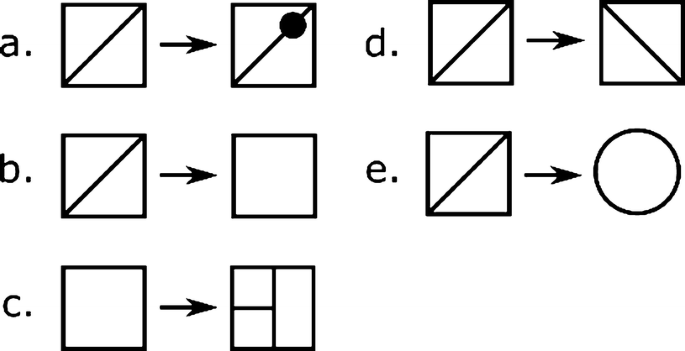
\includegraphics[width=0.85\textwidth]{shape_grammar_fig1.png}
\end{center}

\prop{5.31}{t}{Grammatikkoperasjonen er ein C\msym{→}C-partisjon; ho utvidar tanken. Realisering er ein C\msym{→}K-operasjon; ho avgjer han. Grammatikken definerer moglegheitsrommet; landskapet fastset trajektorien. Agenten forløyser konfigurasjonen som mest radikalt reduserer lokal spenning.}

\prop{5.4}{d}{Substratet fungerer som ein \textit{null-ordens agent}. Det vetoar konfigurasjonar og gjev resonans til andre gjennom ufravikelege avgrensingar.}

\prop{5.41}{i}{Biologisk vev navigerer via bioelektrisk polarisering;\textsuperscript{22,\,24} menneskeleg praksis via materiell friksjon; ein slimsopp via oscillerande samandragingar; ein språkmodell via vektoriell merksemd. Navigasjonsmekanikken er universell; kompetansen formelt ekvivalent.}

\prop{5.5}{t}{Navigasjonskompetanse akkumulerer seg som strukturert informasjon. Læring er den irreversible ekspansjonen av tilgjengeleg formrom.}

\prop{5.6}{d}{\textbf{Omhug}\textsuperscript{23} er mengda av aksar i formrommet agenten \textit{aktivt} representerer og justerer for. Omhug er ikkje det same som kapasitet. Kapasiteten er bredda på lyskjegla; det er kor mange aksar agenten \textit{kan} representere. Omhugen er kor mange han faktisk representerer.}

\prop{5.61}{t}{Agenten navigerer berre innanfor lyskjegla. Omhugen avgjer kor mange aksar lyskjegla rommar. Ein agent med omhug for tre dimensjonar oppdagar kompromiss ein agent med éin dimensjon ikkje veit finst. Den fyrste produserer former som toler fleire trykk samstundes. Den andre produserer former som sviktar langs dei aksane ho ikkje såg.}

\prop{5.62}{d}{Kompetansen til ein agent er evna til å navigere mot stabile posisjonar i landskapet. Kompetansen veks med omhugen. Det me kallar intelligens, er nettopp denne kompetansen. Omhug er difor intelligensen sitt innhald; intelligens er omhugen si form.\textsuperscript{23}}

\prop{5.63}{t}{Ein agent utan omhug for ein dimensjon er blind for landskapets gradient langs den aksen. Blindskapen er ikkje nøytral. Dei usynlege trykka verkar framleis. Forma som oppstår under redusert omhug ber signaturen av det agenten ikkje såg; ho sviktar der ho aldri vart prøvd. Omhugen kan ikkje supplerast i ettertid; den måtte vore der då forma vart navigert.}

\prop{5.64}{a}{Å utvide lyskjegla er ei etisk handling. Premissen kviler på at designhandlinga har reelle konsekvensar for andre agentar som navigerer det same landskapet. Å snevra ho er å overlevere delar av formverda til krefter ingen representerer. Konsekvensane er borna av dei som lever med forma, ikkje av den som formgav ho.}

\flowchapter{6 Forma oppstår mellom agentane}{forma oppstår mellom agentane}

\mainprop{6}{}{Forma oppstår i feltet mellom agentar.}

\prop{6.1}{t}{Fleire agentar responderer på ulike trykk samstundes. Kvar form er eit \textit{poly-agentisk kompromiss}. Ingen einskild agent dikterer morfologien; ho trer fram i skjeringspunktet mellom dei.}

\prop{6.11}{t}{Kvart nivå løyser problem kompetent innanfor si eiga lyskjegle. Lågare komponentar fremjar mål dei manglar kapasitet til å representere. Reduksjonisme og holisme er komplementære; begge er sanne, ingen er tilstrekkeleg åleine.}

\prop{6.12}{t}{Agens er \textit{multiskalar}.\textsuperscript{22} Kvar skala har sin eigen kompetanse og si eiga lyskjegle. Formproduksjon er distribuert C\msym{↔}K-ekspansjon utført av grammatikkoperasjonar over kompetanseskalaer.}

\propcont{Formelt. Form = SG(\,\msym{∇}\textsubscript{C(A)}\, L(\textit{c},\,\textit{t}\,)\,), der SG er grammatikken, \msym{∇}\textsubscript{C(A)} er gradienten avgrensa til lyskjegla, og L er landskapet. Forma er grammatikkens respons på den gradienten agenten kan sjå.}

\prop{6.13}{t}{Agenten vel; landskapet filtrerer. Kontrollen er alltid delt. Utforsking krev lause koplingar; utnytting krev tette.}

\prop{6.14}{t}{Designaren er aldri åleine i landskapet. Ho navigerer i eit felt av konkurrerande agens frå mikrobielt vev til marknadskrefter. Kompetansen hennar ligg i å koordinere uavhengige lyskjegler til eit stabilt form-optimum.}

\prop{6.2}{o}{Tett samanbinding etablerer globale tilbakekoplingssløyfer; heilskapen vert sjølv ein agent.}

\prop{6.3}{t}{Ein \textit{stilart} manglar kausal kraft;\textsuperscript{9,\,15} han er ikkje ei kraft, men eit \textit{mønsterminne}. Stilarten fungerer som ein makroskala-attraktor som kanar lyskjeglene til agentane som observerer han.}

\propcont{Han forenklar navigasjon ved å tilby eit gjenkjenneleg tyngdepunkt; men å formgje «i ein stil» utan å forstå trykka som genererte klynga, er ein kategorifeil.}

\propcont{Å velje medvite frå historia sine former er derimot ein kompetanse: designaren som navigerer med stilkunnskap representerer fleire aksar enn den som navigerer utan.}

\prop{6.31}{o}{Brukaren navigerer formverda gjennom stil. For brukaren er stilarten ikkje eit symptom; han er eit grensesnitt. Brukaren persiperer ikkje seleksjonstrykka; ho persiperer tyngdepunktet. Designaren som ignorerer dette, ignorerer agenten ho formgjev for.}

\prop{6.4}{t}{Kvar realisert form viser agentane at posisjonen er mogleg; ho utvidar det kjende og forskyver grensa til det nærliggande moglege. Formhistoria tømmer ikkje eit lukka repertoar; ho utvidar det gjennom rørsle.}

\prop{6.5}{t}{Inga form er endeleg. Kvar balanse vert med tida suboptimal. Berre den generative strukturen varer; formrom, trykk, landskap, agentar. Formene er flyktige spor; grammatikken er stabil.}

\prop{6.6}{o}{Formverda er det tilfellet som verkar. Navigasjonen held fram. Denne traktaten er sjølv ein posisjon i formrommet; ho er falsifiserbar.}

\flowchapter{7}{forma viser kor langt omhugen rakk}
\mainprop{7}{}{Forma viser kor langt omhugen rakk.}

\prop{7.1}{t}{Den realiserte forma er eit leseleg arkiv over kompromisset sin dimensjonalitet. Ei form designa under trong omhug sviktar systematisk langs dei aksane som ikkje vart tekne vare på. Svikten er ikkje tilfeldig; ho ber signaturen av blindskapen som produserte ho. Påstanden er deskriptiv og falsifiserbar uavhengig av den normative.}

\prop{7.2}{a}{Dersom designaren kunne ha representert fleire aksar men valde å ikkje gjere det, er dei resulterande sviktane tilskrivbare det valet. Premissen er at agentar bør representere so mange aksar som dei har kapasitet til. Premissen er ikkje deduserbar frå dei føregåande proposisjonane; men han er heller ikkje vilkårleg. Han følgjer av at designhandlinga har reelle konsekvensar for andre agentar.}